\part{ÉTAT DE L’ART}
\chapter{PRÉSENTATION DU PROJET}

\textit{Dans ce premier chapitre de la première partie de notre mémoire, nous allons présenter
	notre projet, du contexte à la problématique sans bien sûr oublier les méthodes. Il présente
	notre projet dans son ensemble, il présente la délimitation du sujet, les problèmes à résoudre,
	l’intérêt du sujet et une étude de l’existant.}

\clearpage

\section{Compréhension du sujet}

\subsection{Context}

L’apprentissage est un ensemble de mécanismes menant à l'acquisition de savoir-faire, de savoirs ou de connaissances afin de s’en servir dans la vie courante ou de les faire évoluer pour les générations futures. Malgré les évolutions technologiques offrant de nouvelle façon d’acquérir des connaissances, le système éducatif africain plus précisément camerounais n’a pas beaucoup évoluer les moyens de dispenser les connaissances ne suivent pas toujours les tendances actuelles. Les personnes apprennent mieux en s’immergent dans ce qu’ils font qu’en le théorisant, cela est toujours possible dans le processus d’apprentissage mais pas dans tous les domaines de formation du fait des risque lié à l’acquisition des connaissances en pratique.

Parmi ces domaines ou l’immersion réel des apprenant dans les conditions réels de pratique présente des risques réel pour l’apprenant nous pouvons parler de la chimie, qui est un domaine de la science très expérimentale nécessitant des observations pour une compréhension du sujet étudié en vue d’y apporter des applications dans la vie courante. Une grande et bonne compréhension de ce domaine pourrait apporter de nombreuses idées de recherche qui permettront des avancées significatives dans de nombreux domaines (agriculture, industrie, mode, la mécanique, l'énergie…), avancées qui pourraient à leur tour faciliter le processus d'émergence en Afrique et plus précisément au Cameroun. Malgré l’aspect très expérimentale de son apprentissage, il reste assez dangereux et couteux à enseigner en pratique, dangereux car le manque d’expérience des apprenant pourrais les pousser à commettre des erreurs qui pourrait causer des accidents très dangereux voire mortelle en fonction des éléments manipulés et couteux car la maintenance du matériel nécessaire aux expérimentations (local, verrerie, éléments et personnelles de maintenance) engendre des coûts assez élevé.

\textbf{VREDU} est une plateforme dont l’objectif est de limiter les coûts et les risques lors des expérimentations en concevant le réalisme afin de créer un sentiment d’immersion pour une meilleure compréhension. Pour ce faire monglo technology s’est intéressé à la réalité virtuelle qui est une expression désignant les dispositifs permettant de simuler numériquement un environnement par la machine (ordinateur), afin d’apporter ce réalisme et limiter les risques d’accident.

\subsection{Délimitation du sujet et hypothèse du travail}

Notre travail se limitera au cas de la chimie.

\begin{itemize}
	\item Création des réactions chimique
	\item Expérimentation des réactions dans un environnement immersif
\end{itemize}

\section{Étude de l’existant}

L’étude de l’existant a pour but d'approfondir l'analyse des axes innovants d'un projet au cours d'élaboration, et avant sa mise en œuvre. Cette étude préalable sert à donner un aperçu sur la pertinence du projet, sa faisabilité ainsi que sa continuité.

\subsection{Description de l’existant}

Nous ne saurions débuter ce travail sans avoir une idée claire et précise sur l’existant quel qu’il soit. Dans la plupart des lycées, l’enseignement de la chimie suit un modèle traditionnel à savoir, cours théoriques en salle de classe au cours duquel l’apprenant découvre les principes théoriques nécessaire à la maitrise de cette science. Ensuite un cours pratique en laboratoire au cours duquel les apprenants découvrent la réalité des réaction grâce aux expérience scientifiques.


\subsection{Critique de l’existant et Problématique}

Au cours de notre étude de l’existant, nous avons pu ressortir de nombreux problèmes liés à la réalisation des réactions dans un environnement réel, parmi lesquelles :

\begin{itemize}
	\item Les risques d’accident au cours d’expérimentation trop élevé dans un environnement réel accident qui peut s’avérer mortel suivant les éléments manipulés.
	\item Les coûts de maintenance des équipements qui avec le temps se détériore et nécessite d’être renouvelé ou entretenu régulièrement ce qui entraine des couts matériels et humain assez important.
\end{itemize}

Ceci nous à poussé à soulever la provlématique : \textbf{\og Comment l’utilisation des technologies informatiques pourrait-elle contribuer à faciliter l’enseignement de la chimie dans notre système éducatif plus précisément dans l’enseignement secondaire ? \fg} Autrement dit, pourrait–on envisager une plateforme permettant la simulation d’un laboratoire de chimie en limitant les risques d’accident au cours des expérimentations et aussi en limitant les coûts de maintenance du matériel une fois l'environnement fonctionnel ?

\subsection{Quelques solutions existantes}

Il est question ici de noter les points forts de ces dernières et leurs points faibles afin d’ajuster nos objectifs.

\begin{itemize}
	\item \textbf{ONTOP DUO MEAC}

	      Ontop duo meac est une technologie de simulation de vol utilisé dans les écoles d’aviation utilisé par les formateurs pour mettre en pratique les aspects théoriques abordés durant les formations. En effet dans le domaine de l’aviation les simulateurs de vol comme celui-ci sont presque incontournables car en cas d’accident en condition réel dû au manque d’expérience des apprenants, les nombreuses vies seront menacées et des équipements très coûteux seront détruit.

	      Le dispositif est composé d’écran disposés à 180° autour de l’apprenant afin de simuler le point de vue d’un pilote et d’un cockpit fidèle à leur homologue réel.

	      \begin{figure}[H]
		      \centering
		      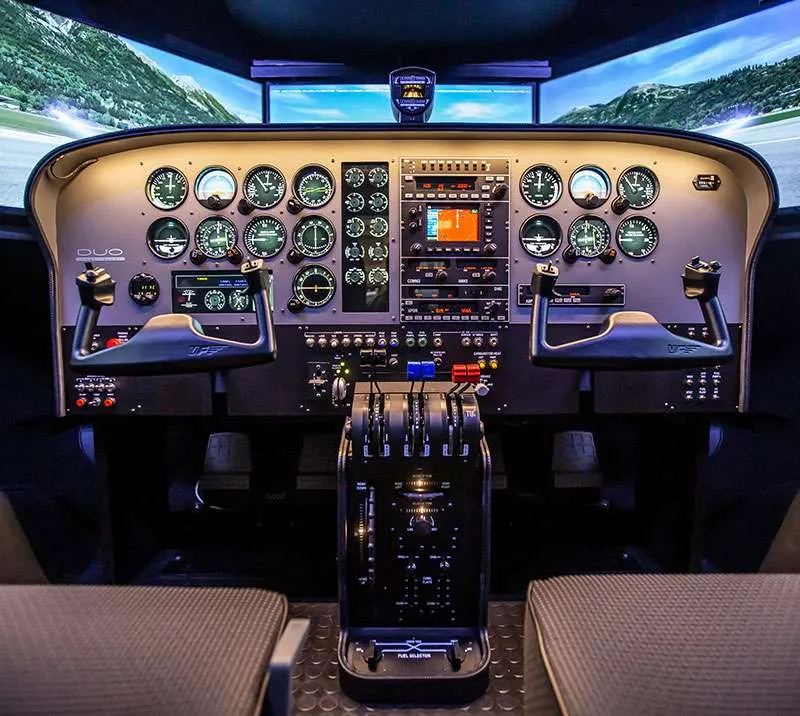
\includegraphics[width=0.5\textwidth]{img/svol1}
		      \caption{Simulateur de vol ONTOP DUO MEAC}
		      \label{fig:mesh1}
	      \end{figure}

	\item \textbf{Microsoft flight simulator}

	      Flight Simulator est un logiciel de simulation de vol pour Microsoft Windows, vendu et souvent vu comme un jeu vidéo. Tout comme le Ontop duo meac, il permet à l'apprenant de comprendre le domaine de l’aviation en pratiquant à moindre coût car il n’a besoin que d’une console de jeu (PlayStation, Xbox, ...) et de contrôleurs, ici des manettes des consoles ou des dispositifs spéciaux.

	      Cette technologie est beaucoup moins rependue dans les centres de formation, car elle est plus adaptée pour les apprenants désireux de s’entrainer chez eux et ne disposant pas des moyens pour un Ontop duo meac.

	      \begin{figure}[H]
		      \centering
		      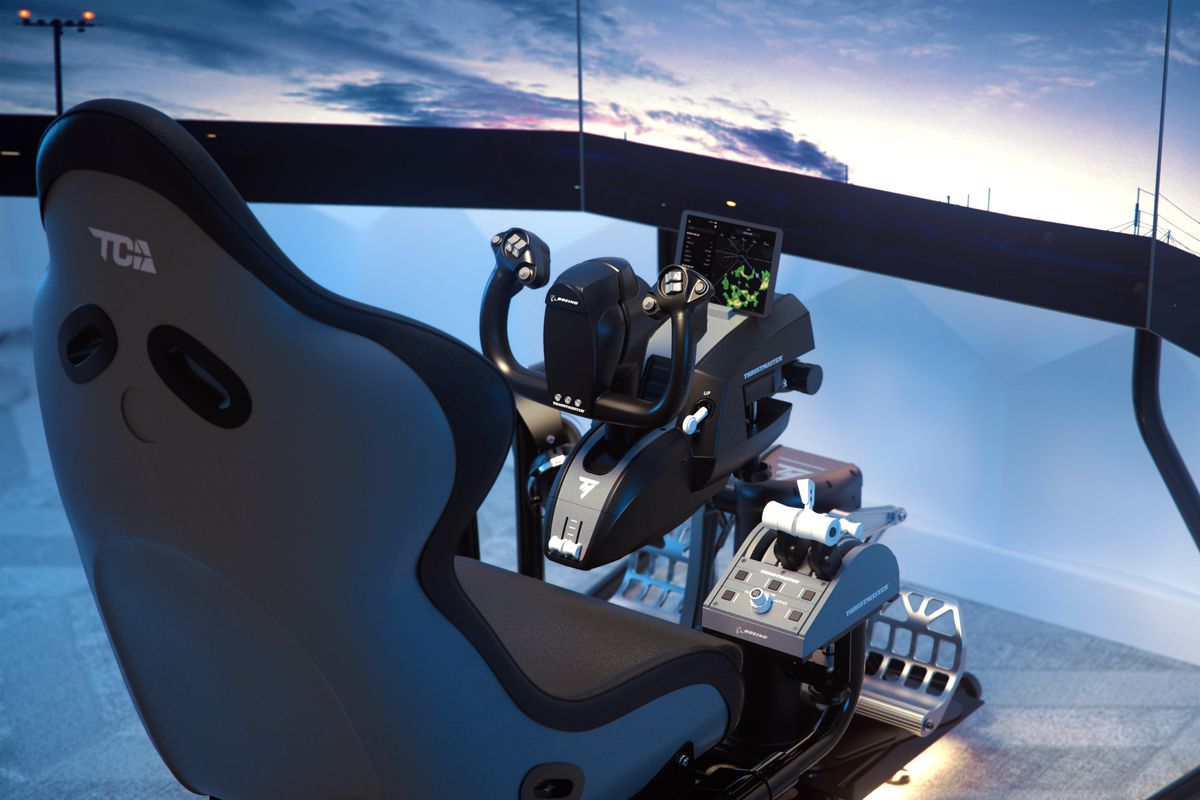
\includegraphics[width=0.5\textwidth]{img/svol2}
		      \caption{Simulateur de vol Microsoft flight simulator}
		      \label{fig:mesh1}
	      \end{figure}

	\item \textbf{Osso VR}

	      Osso VR est une plateforme de formation et d'évaluation chirurgicales qui offre aux entreprises de dispositifs médicaux et aux professionnels de la santé des moyens radicalement meilleurs de partager, de pratiquer. Tout comme dans le domaine de l’aviation, le domaine médical plus précisément chirurgicale utilise des outils de simulation de l’aspect pratique de l’apprentissage. Ceci du au risque lié à l’expérimentation sur des individue vivant et le manque de cadavre.

	      Osso VR utilise la réalité virtuelle pour les expérimentations, afin de simuler un monde en trois dimensions représentant un laboratoire ou est disposé un patient virtuel sur lequel seront effectué les expérimentations.

	      \begin{figure}[H]
		      \centering
		      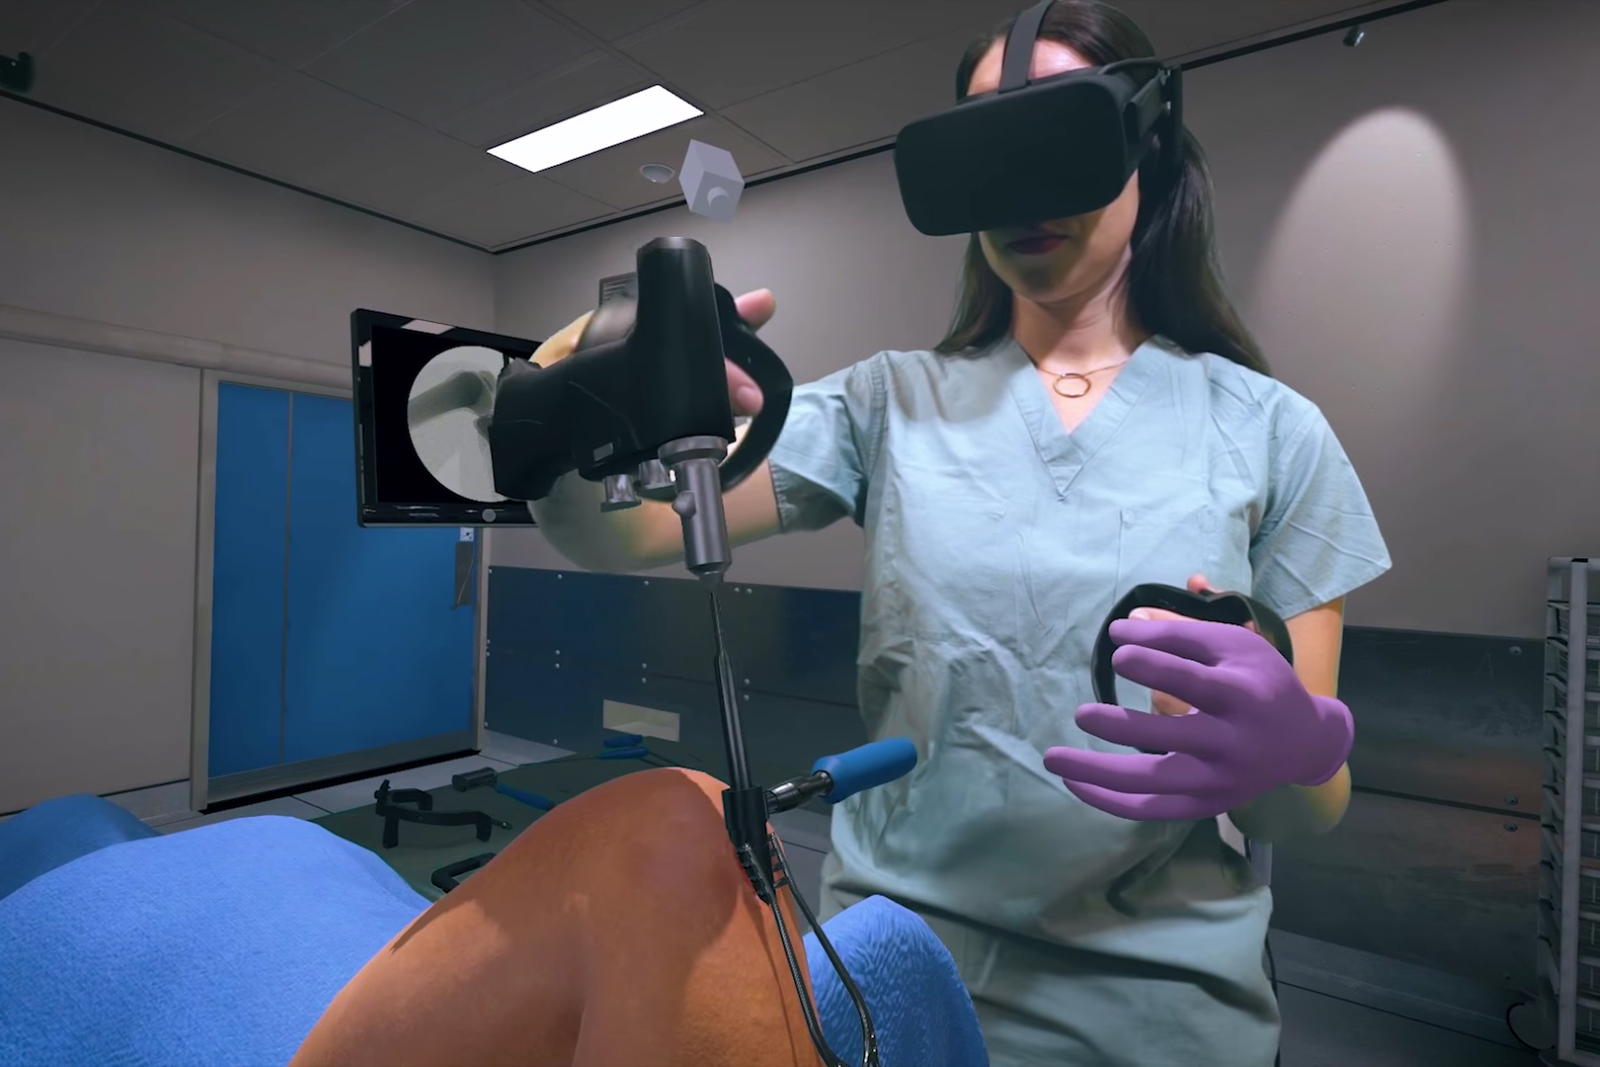
\includegraphics[width=0.5\textwidth]{img/vsurgery}
		      \caption{Simulateur chirurgicale Osso VR}
		      \label{fig:mesh1}
	      \end{figure}

	\item \textbf{Praxilab}

	      Praxilab est un outil didacticiel permettant la simulation d’expérience scientifiques dans les domaines de la biologie, la physique et la chimie. Cet outil est développé pour les plateformes desktop et web et permet aux apprenant de suivre des instructions afin de réaliser des expériences et comprendre des phénomènes liés aux différents domaines.

	      \begin{figure}[H]
		      \centering
		      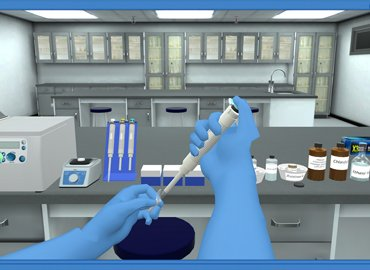
\includegraphics[width=0.5\textwidth]{img/vlab1}
		      \caption{Simulateur scientifique Praxilab}
		      \label{fig:mesh1}
	      \end{figure}

	\item \textbf{EON Reality}

	      EON Reality est une solution de formation académique et industrielle en réalité augmentée et virtuelle. Elle permet l’expérimentation virtuel dans plusieurs domaines de l’enseignement à savoir la mécanique, la chimie, la biologie, l’histoire, le génie civil et plein d’autres domaines.

	      Cette solution est disponible sur de nombreux support à savoir ordinateur sur Windows, casques de réalité virtuelle oculus, sous Android et iOS.

	      \begin{figure}[H]
		      \centering
		      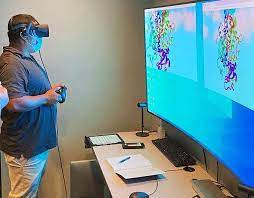
\includegraphics[width=0.5\textwidth]{img/vlab2}
		      \caption{Simulateur scientifique EON RealityC}
		      \label{fig:mesh1}
	      \end{figure}
\end{itemize}

\begin{table}[H]
	\centering
	\caption{Comparatif des solutions existantes}
	\begin{tabular}{|l|p{5cm}|p{5cm}|}
		\hline
		\textbf{Application}       & \textbf{Avantages}                                                                                      & \textbf{Inconvénants}                                                          \\ \hline
		ONTOP DUO MEAC             & Très immercif et réaliste, maintenu et populaire dans le milieu de l'aviation.                          & Trop chère pour une utilisation à domicile, pas adapté aux sciences chimiques. \\ \hline
		Microsoft flight simulator & Assez peu chère à l'obtention donc adapté à une utilisation à domicile et maintenu                      & Pas tres immercif et réaliste, pas adapté aux science chimiques                \\ \hline
		Osso VR                    & Immercif, assez réaliste et maintenu                                                                    & Disponible seulement en démo, pas adapté aux science chimiques.                \\ \hline
		Praxilab                   & Assez réaliste, accessible, adapté au expérience chimique et maintenu                                   & Pas tres immercif, impossible de creer des réactions, pas de version francaise \\ \hline
		EON Reality                & immercif, tres polyvalent, disponible sur de nombreuses plateformes et en plusieurs langues et maintenu & impossible de creer des réactions                                              \\ \hline
	\end{tabular}
\end{table}

\subsection{Questions de recherche}

\begin{itemize}
	\item Comment pouvons nous rendre l'enseignement de la chimie moins couteux ?
	\item Comment pouvons nous rendre l'enseignement de la chimie moins risqué ?
	\item Comment concerver l'aspect réaliste et immercif des expérimentations réelles ?
	\item Comment permettre aux enseignants de creer des réactions pour leur expérimentations ?
\end{itemize}

\section{Choix et intérêt du sujet}

Le contexte dans lequel nous nous trouvons et la problématique nous oriente vers un
choix de thème qui est \textbf{\og Analyse et conception d'un module d'apprentissage immersif basé sur la réalité virtuelle : cas de la chimie \fg}.
La plateforme \textbf{VREDU Chemistry lab} permettra non seulement de résoudre le problème lié aux coûts de maintenance
du matériel et des infrastructures en limitant aussi les risques au cours des expérimentations.

\section{Objectif du travail}

L’objectif général est d'apporter un outil d'aide à l'enseignement secondaire plus précisement de la chimie
afin qu'un enseignant puisse créer des réactions que les apprenants suivront durant la phase pratique du cours.

Les objectifs spécifiques sont :

\begin{itemize}
	\item Représentation des réactifs et des produits en trois dimensions et de façon réaliste et immercive
	\item Calcul des quantités de matière des réactifs dans une solution
	\item Calcul de la concentration des réactifs dans une solution
	\item Calcul de la masse molaire moléculaire des réactifs dans une solution
	\item Calcul du ph d’une solution
\end{itemize}

\section{Methodologie}

\subsection{Gestion de projet}

Pour le pilotage de notre projet, nous devons choisir parmi les méthodes de gestion de
projet une qui convient le mieux non seulement à notre projet mais également à notre contexte
en entreprise. Pour ce faire, nous allons dans un premier lieu faire une comparaison de ces
méthodes afin de faire un choix convenable.

Alors que les méthode traditionnelles visent à traiter les différentes phases d’un projet d’une
manière séquentielle (que l’on nomme aussi cycle de développement en cascade ou encore cycle
en V ), le principe des méthodes Agiles est de le découper en sous-parties (ou sous-projets)
autonomes (on parle également de développement itératif). Les parties (itérations) forment le
projet dans sa globalité.

Nous allons présenter dans un tableau une étude comparative entre l’approche de gestion
de projet agile et celle traditionnelle.


\begin{table}[H]
	\centering
	\caption{Comparaison entre les approches traditionnelles et agiles}
	\label{tab:my-table}
	\begin{tabular}{|l|p{5cm}|p{6cm}|}
		\hline
		\textbf{Thème}      & \textbf{Approche traditionnelle}                                                                       & \textbf{Approche agile}                                                                                                                                              \\ \hline
		Cycle de vie        & En cascade ou en V, sans rétroactions possible, phases séquentielles                                   & Itératif et incrémental                                                                                                                                              \\ \hline
		Planification       & Produite en quantité importante comme support de communication, de validation et de contractualisation & Réduite au strict nécessaire au profil d’incréments fonctionnels opérationnels pour le feedback du client                                                            \\ \hline
		Equipe              & Contrôle de qualité à la fin du cycle de développement. Le client découvre le produit fini.            & Un contrôle de qualité précoce et permanent au niveau du produit et du processus. Le client visualise les résultats tôt et fréquemment                               \\ \hline
		Qualité             & Une équipe avec des ressources spécialisées, dirigée par un chef de projet.                            & Une équipe responsabilisée ou l’initiative et la communication sont privilégiées soutenu par le chef de projet                                                       \\ \hline
		Suivi d’avancement  & Mesure de la conformité aux plans initiaux. Analyse des écarts.                                        & Un seul indicateur d’avancement : le nombre de fonctionnalité implémentées et le travail restant à faire.                                                            \\ \hline
		Changement          & Résistance voire opposition au changement. Processus lourd de gestion des changement acceptes          & Accueil favorable au changement, intègre dans le processus                                                                                                           \\ \hline
		Gestion des risques & Processus distinct, rigoureux de gestion des risque                                                    & Gestion de risques intégrée dans le processus global, avec responsabilisation de chacun dans l’identification et la résolution des risques. Pilotage par les risques \\ \hline
		Mesure du succès    & Respect des engagements initiaux en termes de coûts, de budget et ce niveau de qualité                 & Satisfaction client par la livraison de valeur ajoutée                                                                                                               \\ \hline
	\end{tabular}
\end{table}

De cette comparaison, il est possible de choisir selon le projet, l’approche qui convient le
mieux.

Au vu de notre projet, il convient pour nous de choisir une méthode agile car cette dernière
s’adapte facilement aux changement et n’impose pas une planification rigide dès le début du
projet. Parmi les méthodes agiles existantes, nous devons en choisir une qui nous convient
encore plus. Après cette comparaison, notre choix s’oriente vers SCRUM. Car au vue de la grandeur de notre projet, de la taille de l’équipe, des préférences de l’entreprise
et de l’approche orientée objet, nous pensons qu’elle est la méthode la mieux adaptée.

\begin{table}[H]
	\centering
	\caption{Comparaison des méthodes agiles}
	\label{tab:my-table}
	\begin{tabular}{|l|l|l|l|}
		\hline
		\textbf{Méthode}                & \textbf{Flexibilité} & \textbf{Itératif} & \textbf{Taille} \\ \hline
		\textbf{Scrum}                  & oui                  & oui               & toute           \\ \hline
		\textbf{Crystal clear}          & oui                  & Non               & petite          \\ \hline
		\textbf{Processus unifié Agile} & oui                  & Non               & toute           \\ \hline
		\textbf{eXtreme Programing}     & oui                  & oui               & petite          \\ \hline
	\end{tabular}
\end{table}

\subsubsection{Qu’est-ce que la Méthode SCRUM}

Scrum est un cadre léger qui aide les personnes, les équipes et les organisations à générer de la valeur grâce à
des solutions adaptatives pour des problèmes complexes\cite{schwaber2011scrum}.

Souvent considéré comme un framework de gestion de projet Agile, Scrum décrit un ensemble de réunions, d'outils et de rôles qui interagissent de concert pour aider les équipes à structurer leur travail et à le gérer.

Scrum est fondé sur l'empirisme et la pensée Lean. L'empirisme affirme que la connaissance vient de l'expérience et de la prise de décisions basées sur ce qui est observé. La pensée Lean réduit le gaspillage et se concentre sur l'essentiel\cite{schwaber2011scrum}.

Scrum utilise une approche itérative et incrémentale pour optimiser la prévisibilité et contrôler les risques. Scrum engage des groupes de personnes qui ont collectivement toutes les compétences et l'expertise pour faire le travail et partager ou acquérir ces compétences selon les besoins. Scrum combine quatre événements formels pour l'inspection et l'adaptation dans un événement conteneur, le Sprint. Ces événements fonctionnent parce qu'ils mettent en œuvre les piliers empiriques de Scrum que sont la transparence, l'inspection et l'adaptation.

\vspace{1em}
\begin{itemize}
	\setlength\itemsep{1em}
	\item \textbf{La transparence}: La Transparence est un facteur clé de réussite. Tout au long du développement du produit, l’équipe de développement et les parties prenantes ont accès aux informations basées sur un langage et des définitions communs . Par exemple, la définition de fini (DOD, definition of done) est très importante et obligatoire pour Scrum. La définition de prêt (DOR, definition of ready) est aussi une pratique couramment utilisée mais non obligatoire à ce jour si on se réfère au Scrum Guide.
	\item \textbf{L'inspection et l'adaptation} : L’équipe doit se consulter quotidiennement pour détecter rapidement d’éventuels écarts entre l’objectif de l’itération(Sprint Goal) et le travail réalisé. Cette Inspection dans le Sprint a lieu principalement lors du Daily Scrum, de la Sprint Review et de la Sprint Retrospective. Si des écarts sont constatés, un ajustement doit être entrepris afin d’atteindre les objectifs du Sprint.

	      L’Inspection et l’Adaptation permettent d’ajuster en permanence le développement d’un produit en fonction de l’apprentissage réalisé lors de chaque itération.
\end{itemize}

\subsubsection{Pourquoi la méthode SCRUM}

Cette méthode permet de répondre aux besoins des utilisateurs rapidement, dans les délais
impartis, tout en respectant les budgets. En effet, elle canalise et modélise toutes les étapes du
développement d’un logiciel. Elle ordonne aussi très clairement les différents jalons.

\subsubsection{Avantages de la méthode SCRUM}

Les équipes qui optent pour la structure Scrum gagnent en agilité et en flexibilité. Elle contribue à renforcer la collaboration au sein des équipes et les aide à atteindre leurs objectifs plus efficacement. Par ailleurs, les équipes Scrum savent en permanence sur quoi elles travaillent : elles accomplissent des tâches de leur backlog produit et ont une idée claire de leurs objectifs, car elles se sont concertées sur la définition d’un travail \og terminé \fg.

\subsubsection{Dans quels cas utiliser la méthode SCRUM}

Offrant plus de réactivité, elle est plus adaptée que les méthodes traditionnelles pour la gestion de projets web, tel que le développement logiciel, car elle traduit et organise les projets de façon simple, transparente et pragmatique.

Ce framework, ou cadre de travail, est utile quand :

\vspace{1em}
\begin{itemize}
	\setlength\itemsep{1em}
	\item L’ensemble d’un projet complexe ne peut être ni anticipé ni planifié entièrement.
	\item Son pilotage demande un minimum de flexibilité pour intégrer facilement des changements aux planifications initiales.
\end{itemize}

\subsubsection{Principale contrainte de la méthode SCRUM}

Les projets Scrum souffrent souvent de dérives des objectifs, car cette méthode accepte et encourage le changement. Cependant, il présente des risques d’itérer sans obtenir de résultats concrets si les changements sont trop nombreux ou que les retours clients sont discordants.

\subsection{Analyse et Modélisation}

Pour la réalisation du projet nous allons procéder comme suit :

\vspace{1em}
\begin{itemize}
	\setlength\itemsep{1em}
	\item Séparation des différents modules à déployer
	\item développer les différents en utilisant l'approche de développement orienté objet
	\item Déployer ces modules pour la production
\end{itemize}

\subsubsection{L’approche orientée objet}

L’approche orientée objet considère le logiciel comme une collection d’objets dissociés,
identifiés, et définis par des propriétés. Une propriété est soit un attribut, soit une méthode.
La fonctionnalité du logiciel émerge alors de l’interaction entre les différents objets qui le
constituent. L’une des particularités de cette approche est qu’elle rapproche les données et
leurs traitements associés au sein d’un unique objet. Un objet est caractérisé par plusieurs
notions dont :

\vspace{1em}
\begin{itemize}
	\setlength\itemsep{1em}
	\item \textbf{L’identité} : L’objet possède une identité, qui permet de le distinguer des autres objets, indépendamment de son état. On construit généralement cette identité grâce à un identifiant
	      découlant naturellement du problème (par exemple une Banque pourra être repéré par un code,
	      un Encaissement par un numéro identifiant ... etc.)
	\item \textbf{Les attributs} : Il s’agit des données caractérisant l’objet. Ce sont des variables stockant des
	      informations sur l’état de l’objet.
	\item \textbf{Les méthodes} : Les méthodes d’un objet caractérisent son comportement, c’est-à-dire l’ensemble
	      des actions (appelées opérations) que l’objet est à même de réaliser. Ces opérations permettent
	      de faire réagir l’objet aux sollicitations extérieures (ou d’agir sur les autres objets). De plus, les
	      méthodes sont étroitement liées aux attributs, car leurs actions peuvent dépendre des valeurs
	      des attributs, ou bien les modifier.
\end{itemize}

La difficulté de cette modélisation réside dans la création d’une représentation abstraite, sous
forme d’objets, d’entités ayant une existence matérielle (Exemple : Banque, Guichet, Caisse ...
etc.) ou bien virtuelle (Exemple : Encaissement, Décaissement, Transfert de fonds ... etc.).
La Conception Orientée Objet (COO) est la méthode qui conduit à des architectures logicielles
fondées sur les objets du système, plutôt que sur la fonction qu’il est censé réaliser.

\subsubsection{UML et MERISE}

Les différences entre l’approche objet avec UML et l’approche systémique (fonctionnelle)
avec Merise sont mises en évidence dans l’étude comparative ci- dessous :

\vspace{1em}
\begin{itemize}
	\setlength\itemsep{1em}
	\item \textbf{Points communs}:

	      L’approche classique et l’approche objet distinguent bien globalement trois grandes étapes
	      ans le processus de conception et de développement d’une solution : l’analyse objet correspond
	      au niveau conceptuel de merise, la conception objet est proche de la modélisation logique et
	      organisationnelle de merise. Et enfin l’implémentation objet correspond à la réalisation dans
	      merise

	      Nous allons reprendre chaque grand niveau de représentation du SI et donner un certain nombre
	      de précisions sur les points communs.

	      Le niveau de l’analyse objet ou le niveau conceptuel : dans les deux approches, la finalité de ces
	      premiers niveaux de description d’un SI est d’appréhender les besoins à satisfaire et donner une
	      description de solutions indépendamment des considérations techniques des niveaux logiciel et
	      physique. Autrement dit les préoccupations traitées sont très proches malgré des concepts pas
	      complètements identiques au niveau conceptuel et au niveau de l’analyse objet.

	      Le niveau conception Objet ou le niveau logique-Organisationnel : ce niveau de description a
	      bien pour finalité dans les deux approches de représenter la solution à implémenter sous l’angle
	      de la logique informatique tant sur la partie des données que sur celle des traitements.
	      Le niveau implémentation physique ou opérationnel dans les deux approches la préoccupation
	      est la description physique et opérationnelle des données et traitements.

	\item \textbf{Différences} :

	      Nous observons les différences entre ces deux approches au niveau des domaines d’application,
	      de la démarche, les données et les traitements puis l’aspect évolution du système.

	\item \textbf{Les domaines d’application} :

	      Merise a pour vocation de traiter les systèmes d’informations des entreprises, principalement
	      dans le domaine de l’informatique de gestion. Le domaine de l’informatique de gestion se
	      caractérise en général par un grand nombre de données à gérer et à stocker avec des traitements
	      relativement peu complexes.

	      Le domaine privilégié par UML est le domaine de l’informatique technique ou industrielle
	      caractérisé par la gestion de composants physiques du monde réel (Informatisation des automates
	      est représentatif de ce domaine). Dans ce type de domaine les aspects traitements d’états et
	      comportements des objets, prend le pas sur la gestion des données. En plus de cet atout UML
	      traite également sans difficulté majeur le domaine tel que l’informatique de gestion.

	\item \textbf{La démarche}

	      Avec merise la démarche est structurée en étapes et phases dont l’étude préalable, l’étude
	      détaillée, la réalisation et la mise en œuvre[7]. Il correspond en effet au cycle de vie d’un système
	      d’information. Et l’ensemble des résultats produits à chaque étape constitue le cycle de décision.
	      Merise propose donc une démarche en cascade, c’est-à-dire qu’une étape ne peut être entamée
	      que si l’étape précédente est achevée. Cela nécessite une organisation minutieuse du projet.
	      Dans Je cas contraire l’on pourrait noter quelques blocages ou une lenteur dans le processus
	      de modélisation du système d’information. Avec UML, la démarche est itérative, incrémentale
	      guidée par les besoins des utilisateurs du système, et centrée sur l’architecture logicielle. La
	      démarche itérative permet de mieux comprendre et représenter un système complexe. Le
	      périmètre du système à modéliser est défini par les besoins des utilisateurs (les utilisateurs
	      définissent ce que doit être le système).

	\item \textbf{Choix d’une méthode d’analyse}

	      Suite à notre étude comparative entre l’approche systémique avec Merise et l’approche Objet
	      avec UML, Nous opterons donc pour une méthode d’analyse suivant l’approche Objet dont UML
	      pour la modélisation, dans l’étude conceptuelle de notre système. Ensuite vue les circonstances
	      et les délais de notre projet nous optons pour une démarche itérative, incrémentale guidée par
	      les besoins des utilisateurs du système. De plus nous souhaiterions organiser nos programmes
	      en rassemblant les données et les traitements en vue de for mer des entités cohérentes, logiques
	      et stables. Enfin nous aimerions faciliter les éventuelles évolutions et maintenances du système.
\end{itemize}